\chapter{Einleitung}

Die Einkommensverteilung ist ein zentraler Aspekt einer jeden Wirtschaft und spielt eine bedeutende Rolle in der Beurteilung der wirtschaftlichen Chancengleichheit einer Gesellschaft. In Deutschland ist sie zudem ein Thema von gro{\ss}er gesellschaftlicher und medialer Bedeutung. Gleichzeitig ist die Einkommensverteilung eines Landes ein wichtiger Indikator für soziale Kohäsion und Stabilität. In der heutigen globalisierten Welt führen strukturelle Veränderungen und wirtschaftliche Entwicklungen immer wieder zu Verschiebungen in der Einkommensverteilung, die sowohl national als auch international betrachtet werden müssen. Daher ist der Vergleich der Einkommensverteilung in Deutschland mit dem globalen Niveau von hoher Relevanz.

In dieser Arbeit soll die Einkommensverteilung in Deutschland im internationalen Vergleich betrachtet werden. Hierfür werden verschiedene Indikatoren, wie das T10/B50-Verhältnis, der Gini-Koeffizient und der Anteil der Bevölkerung unterhalb der Armutsgrenze, auf deutscher und globaler Ebene herangezogen. Diese Kennzahlen sollen es ermöglichen, die Einkommensverteilung in Deutschland mit der weltweiten Einkommensverteilung zu vergleichen und so ein umfassendes Verständnis über Gemeinsamkeiten, Unterschiede und aktuelle Entwicklungen schaffen. Diese Erkenntnisse sollen mit Erklärungen aus der Literatur angereichert werden.

\chapter{Indikator-basierter Vergleich der Einkommensverteilungen}

Im Folgenden soll die Einkommensverteilung in Deutschland mit der weltweiten Einkommensverteilung anhand mehrerer Indikatoren verglichen werden. Die Kennzahlen eignen sich besonders, da das T10/B50-Verhältnis die äu{\ss}eren Bereiche des Einkommensspektrums betrachtet, der Gini-Koeffizient ein allgemein etablierter Indikator für die Einkommensverteilung eines Landes ist und die Armutsquote einen Einblick gibt, wie viele Menschen in einer finanziell prekären Situation leben. Durch die Auswertung dieser Indizes soll ein umfassendes Verständnis über die Einkommensverteilung Deutschlands im weltweiten Vergleich geschaffen werden.

\section{T10/ B50 Einkommensverhältnis}

Zuerst wird das gewichtete Verhältnis des Einkommensanteils der reichsten 10\% zum Einkommensanteil der ärmsten 50\% betrachtet (im Folgenden als ''T10/B50'' abgekürzt). Es gibt an, wie hoch der Anteil der reichsten 10\% am Gesamteinkommen im Vergleich zu den ärmsten 50\%, gewichtet nach der absoluten Grö{\ss}e der Gruppen, ist.\footnote{Beispiel: Der Anteil des obersten Dezils am Gesamteinkommen beträgt 50\%, während der Anteil der unteren Hälfte 10\% beträgt. Dann hätte der T10/B50-Indikator den Wert 25, da die Gruppe der unteren 50\% fünfmal so gro{\ss} ist wie die der oberen 10\%.} Je höher der Wert, desto ungleicher sind die Einkommen verteilt. \footcite[Vgl.][S. 31]{wir_2022} 

\begin{figure}[h]
    \centering
    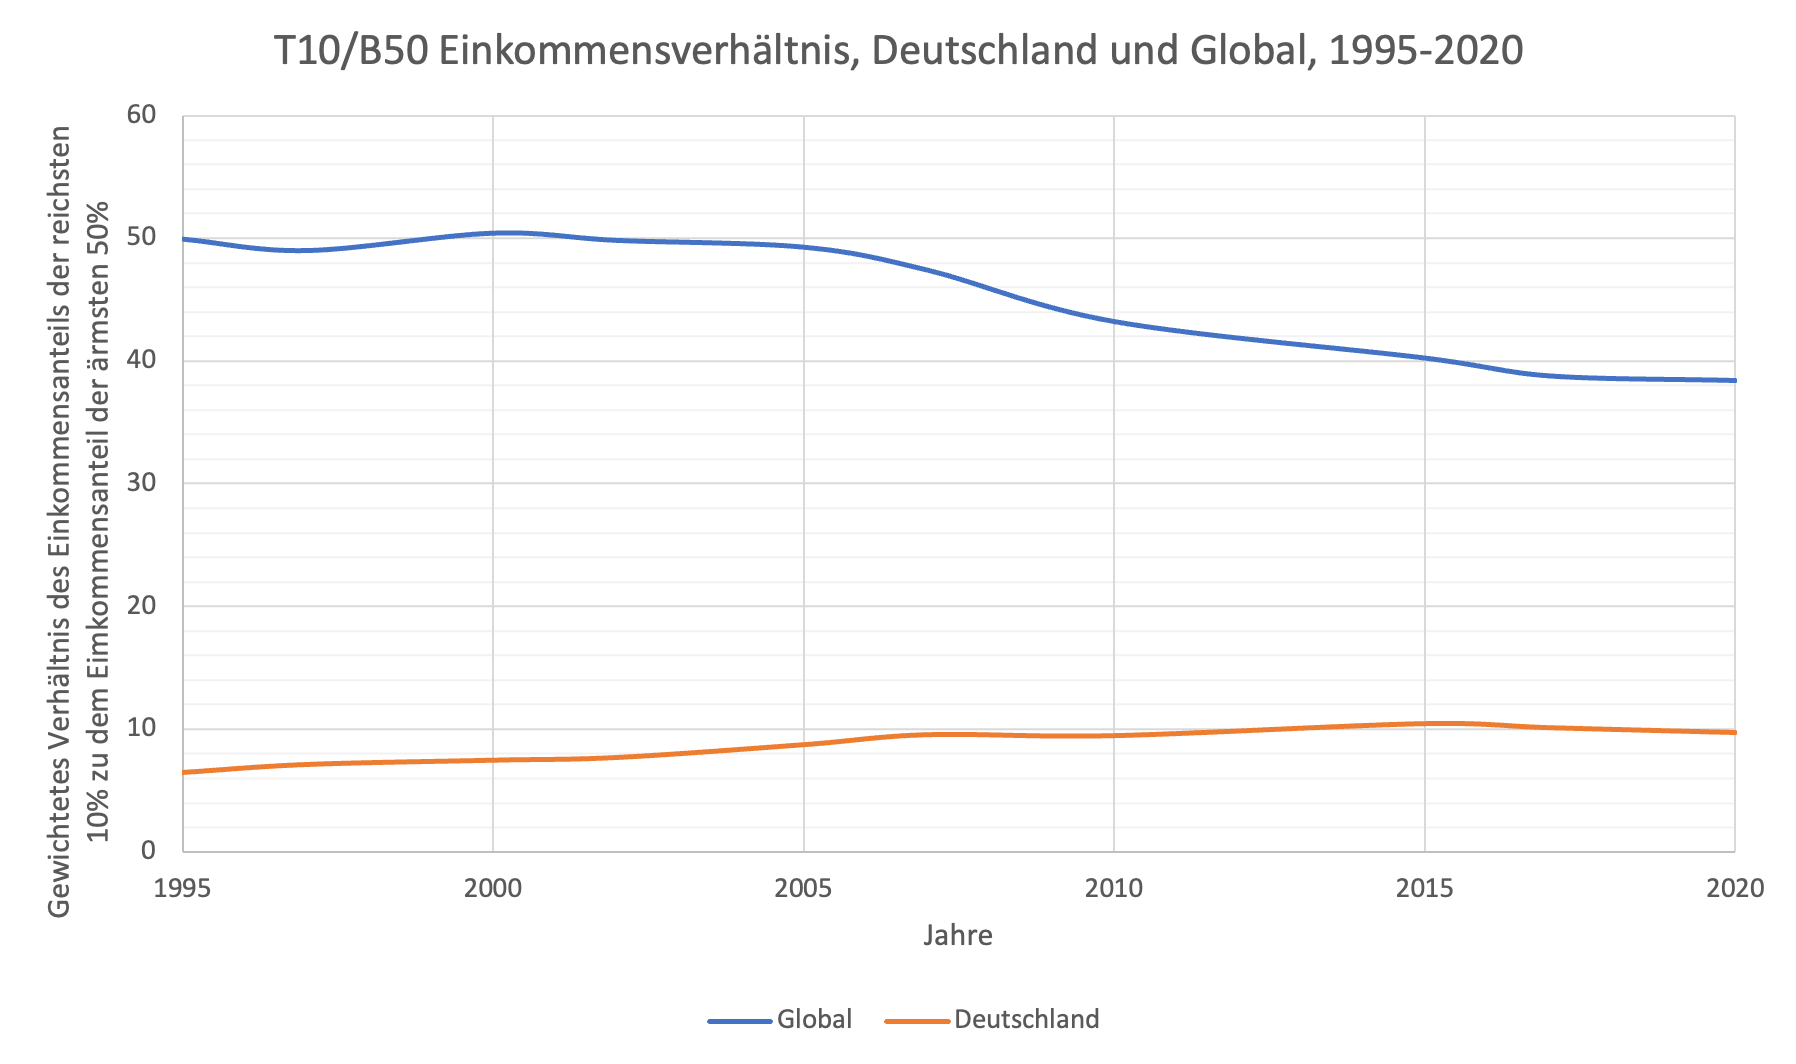
\includegraphics[height=8.15cm]{Bilder/T10B50-Ratio3.png}
    \caption[T10/B50 Einkommensverhältnis, Deutschland und global, 1995-2020]{Gewichtetes Verhältnis des Einkommensanteils der reichsten 10\% zum Einkommensanteil der ärmsten 50\% in Deutschland und auf globaler Ebene von 1995 bis 2020. Eigene Darstellung und Berechnung. Daten abgerufen von \cite[][, S.55, 195]{wir_2022} am 01.03.2024.}
    \label{fig:iso_norm1}
\end{figure}

Anhand der unten abgebildeten Grafik ist zu erkennen, dass das T10/B50-Verhältnis in Deutschland von 1995 bis 2015 von ca. 6 auf 10 stetig angestiegen ist, wohingegen das Verhältnis seit 2015 eher konstant geblieben ist. Somit müssen die Einkommen des obersten Dezils von 1995 bis 2015 stärker gestiegen sein als die Einkommen der unteren Hälfte der Bevölkerung. Nach Daten des DIW sind die Realeinkommen des obersten Dezils in diesem Zeitraum um fast 30\% gestiegen, während die Einkommen der unteren Hälfte nur um ca. 10\% gestiegen sind. \footcite[Vgl.][S. 452]{grabka_einkommensverteilung_2018} Ein möglicher Grund für diese Entwicklung ist unter anderem die gestiegene Arbeitslosigkeit von 2000 bis 2005, die für eine Lohnzurückhaltung gesorgt und die unteren Einkommen stärker getroffen hat. Als weiteren Grund ist die ab 2007 deutlich verstärkte Zuwanderung zu nennen. Diese neu zugezogenen Menschen bräuchten meist mehr Zeit um sich am Arbeitsmarkt zu etablieren und nähmen im Durchschnitt eher niedriger entlohnte Arbeitsstellen an (\cite[Vgl.][S.453]{grabka_einkommensverteilung_2018}). 

Im Gegensatz dazu ist der Indikator auf globaler Ebene im Betrachtungszeitraum von 1995 bis 2005 eher seitwärts entwickelt und ist dann ab 2005 fast konstant von ca. 50 auf 38 gefallen. Dieser Abfall könnte durch die Finanzkrise 2008 und die daraus resultierenden wirtschaftlichen Veränderungen verursacht worden sein. \footcite[Vgl.][S. 55]{wir_2022}

Insgesamt ist festzustellen, dass das T10/B50-Verhältnis in Deutschland im Vergleich zu dem globalen Wert deutlich niedriger ist. Diese Diskrepanz kann durch die in Europa hohen bzw. in Deutschland noch höheren Umverteilungsraten begründet werden. \footcite[Vgl.][S. 36f]{wir_2022} Dennoch hat sich der Abstand zwischen Deutschland und dem globalen Wert in den letzten 25 Jahren von ca. 44 auf 28 verringert, was grö{\ss}tenteils auf einen Rückgang des Indikators auf globaler Ebene, jedoch auch auf einen Anstieg des Indikators in Deutschland zurückzuführen ist. Zusammenfassend lässt sich sagen, dass sich die Einkommensverteilungen in Deutschland und auf globaler Ebene in den letzten 25 Jahren angenähert haben. Die Einkommensungleichheit hat in diesem Zeitraum in Deutschland zugenommen, ist aber immer noch deutlich unter dem internationalen Niveau.

\section{Gini-Koeffizient}

Der zweite herangezogene Indikator ist der Gini-Koeffizient. Er ist ein Ma{\ss} für die Verteilung von Einkommen und Vermögen. Für den Anwendungsfall in dieser Arbeit soll er jedoch nur für die Bewertung der Einkommensverteilung dienen. Er kann Werte zwischen 0 und 1 annehmen, wobei 0 für eine vollkommene Gleichverteilung und 1 für eine vollkommene Ungleichverteilung steht. \footcite[Vgl.][]{gini_definition_diw_2024}

\begin{figure}[h]
    \centering
    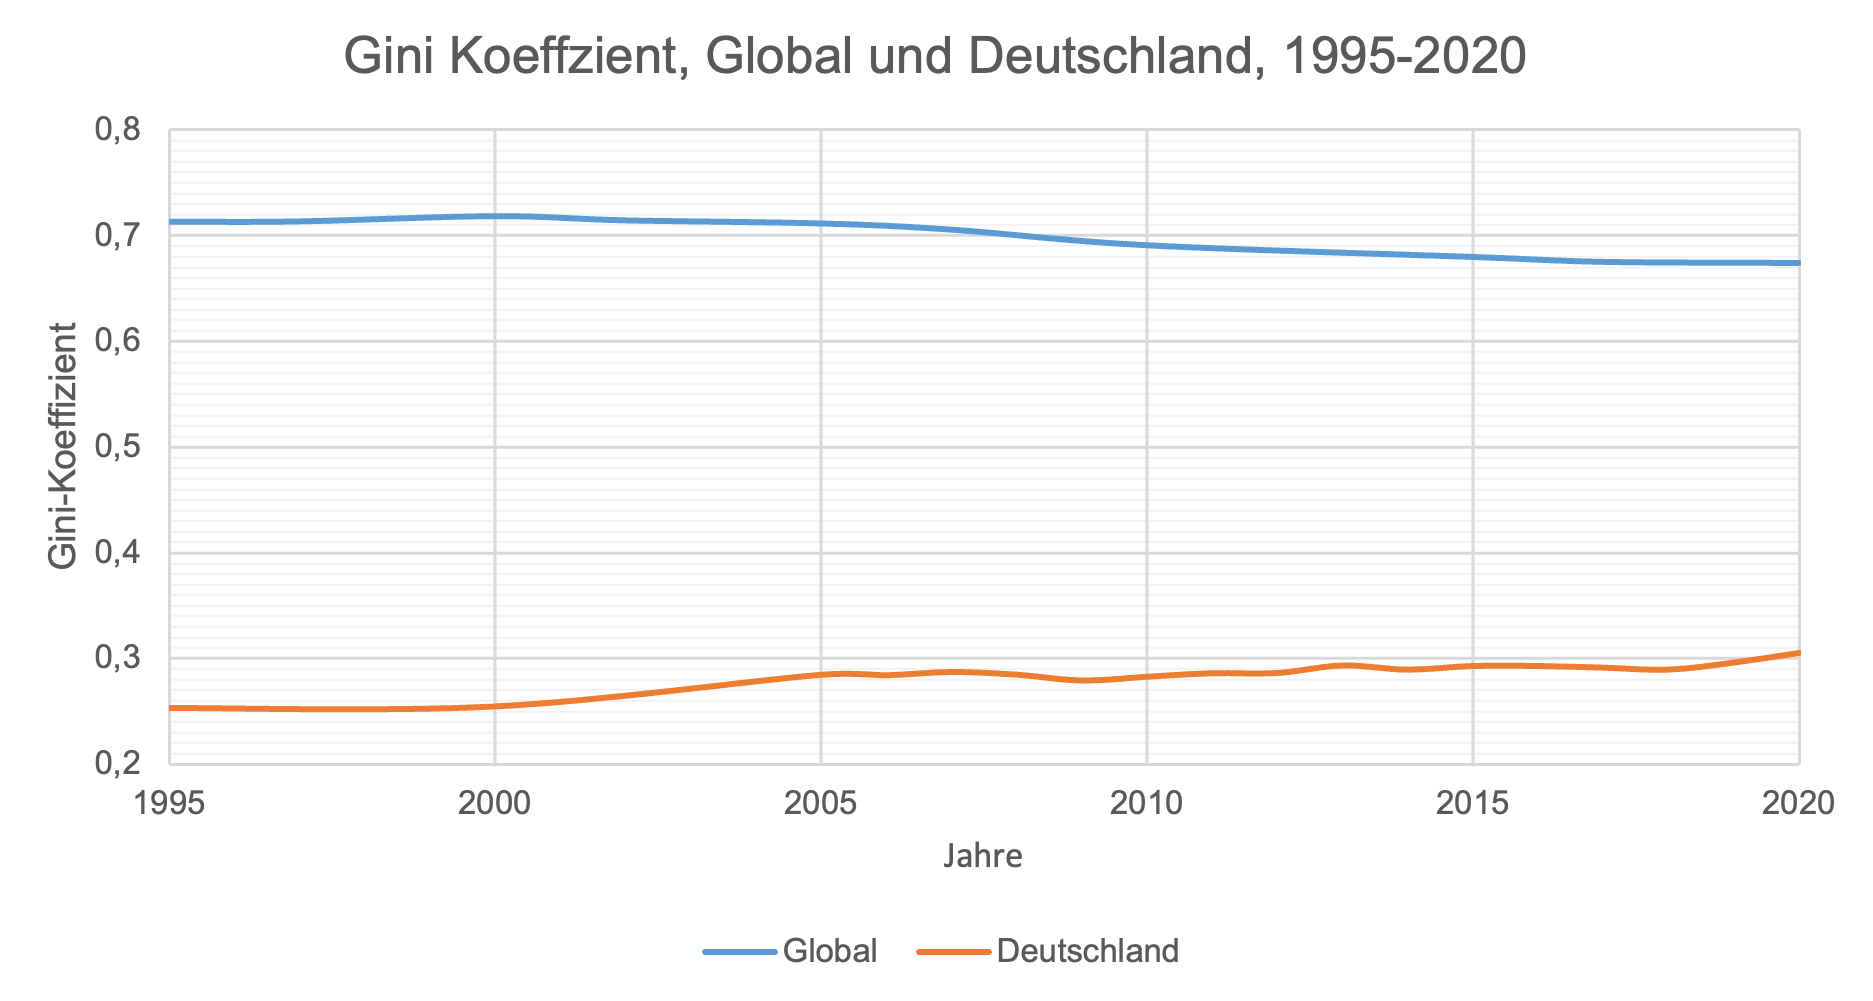
\includegraphics[height=8cm]{Bilder/Gini-Koeffizient2.png}
    \caption[Gini-Koeffizient, Deutschland und global, 1995-2020]{Gini-Koeffizient für Deutschland und auf globaler Ebene von 1995 bis 2020. Eigene Darstellung. Daten abgerufen von \cite[][, S.56 (global)]{wir_2022} und \cite[][(Deutschland)]{bmas_arb_gini_2020} am 01.03.2024.}
    \label{fig:iso_norm2}
\end{figure}

Bei der Betrachtung des Gini-Koeffizienten in Deutschland ist festzustellen, dass dieser über den Betrachtungszeitraum von 0,25 auf 0,31 angestiegen ist. Dieser Anstieg entfällt zu gro{\ss}en Teilen auf das Intervall 2000 bis 2005, während der Gini-Koeffizient im restlichen Betrachtungszeitraum überwiegend konstant geblieben ist. Für den Anstieg des Gini-Koeffizienten Anfang der 2000er-Jahre dürfte, neben den im Vorfeld bereits genannten Gründen, das Platzen der ''Dot-Com''-Blase und die dadurch ausgelöste Wirtschaftskrise verantwortlich sein, die Menschen mit geringeren Einkommen stärker belastet hat. \footcite[Vgl. ][S. 3]{horn_wirtschaftskrise_2014} Bei Betrachtung des gesamten Zeitraums fällt auf, dass sich der Graph des Gini-Koeffizienten mit dem des T10/B50-Verhältnisses ähnelt, was darauf zurückzuführen ist, dass die im oberen Abschnitt beschriebenen Gründe für den Anstieg des T10/B50-Verhältnisses auch den Gini-Koeffizienten beeinflusst haben. Zudem sind beide betrachteten Indikatoren ein Ma{\ss} für die Einkommensverteilung und entwickeln sich aufgrund ihrer Natur ähnlich. Die Tatsache, dass sich beide Indikatoren ähnlich entwickelt haben untermauert nochmals die Aussage, dass die Einkommensungleichheit in Deutschland in den letzten 25 Jahren zugenommen hat.

Die globale Entwicklung des Gini-Koeffizienten ist gegensätzlich zu der in Deutschland. Von 1995 bis 2005 ist dieser mit einem Wert von 0,71 \pm 0,01 fast konstant geblieben, während der Indikator ab 2005 auf 0,67 gefallen ist. Auch bei diesem Indikator kann die Finanzkrise 2008 als mögliche Ursache für den Abfall des Gini-Koeffizienten genannt werden. \footcite[Vgl. ][S. 55]{wir_2022} Daraus kann man den Schluss ziehen, dass diese Krise auf internationaler Ebene für eine Reduktion der Einkommensungleichheit gesorgt hat, während sie in Deutschland zu einer Zunahme geführt hat.

Zusammenfassend lässt sich sagen, dass der Gini-Koeffizient in Deutschland im Vergleich zum internationalen Niveau niedriger ist. Jedoch kann man - analog zum T10/B50-Verhältnis - beobachten, dass sich die Gini-Koeffizienten von Deutschland und der Welt in den letzten 25 Jahren angenähert haben, wobei der deutsche Index einen Trend nach oben und der globale Index einen Trend nach unten aufweist. Unter der Voraussetzung, dass sich die Entwicklungen der letzten 25 Jahre fortsetzen, ist anzunehmen, dass die Einkommensungleichheit in Deutschland in Zukunft weiter zunehmen wird, während sie auf globaler Ebene weiter abnehmen wird. Trotz dieser Tatsache darf nicht vergessen werden, dass die Einkommensverteilung in Deutschland im internationalen Vergleich durch \zB die ausgeprägten sozialen Sicherungssysteme und die hohe Umverteilung von Einkommen und Vermögen deutlich gleichmä{\ss}iger ist.

\section{Bevölkerungsanteil unterhalb der Armutsgrenze}

Als letzte Kennzahl wird der Anteil der Bevölkerung mit einem Einkommen unterhalb der Armutsgrenze betrachtet. In Deutschland ist die Armutsrisikoquote bei 60\% des Medianeinkommens angesetzt. \footcite[Vgl.][]{bmas_arb_armutsrisikoquote_2023} Für die globale Betrachtung werden die jeweiligen Einkommensgrenzen, die jedes Land für sich definiert hat, verwendet, um die verschiedenen Einkommensniveaus zwischen mehreren Ländern auszuklammern. \footcite[Vgl.][]{wb_armutsquote_global_2022}

\begin{figure}[h]
    \centering
    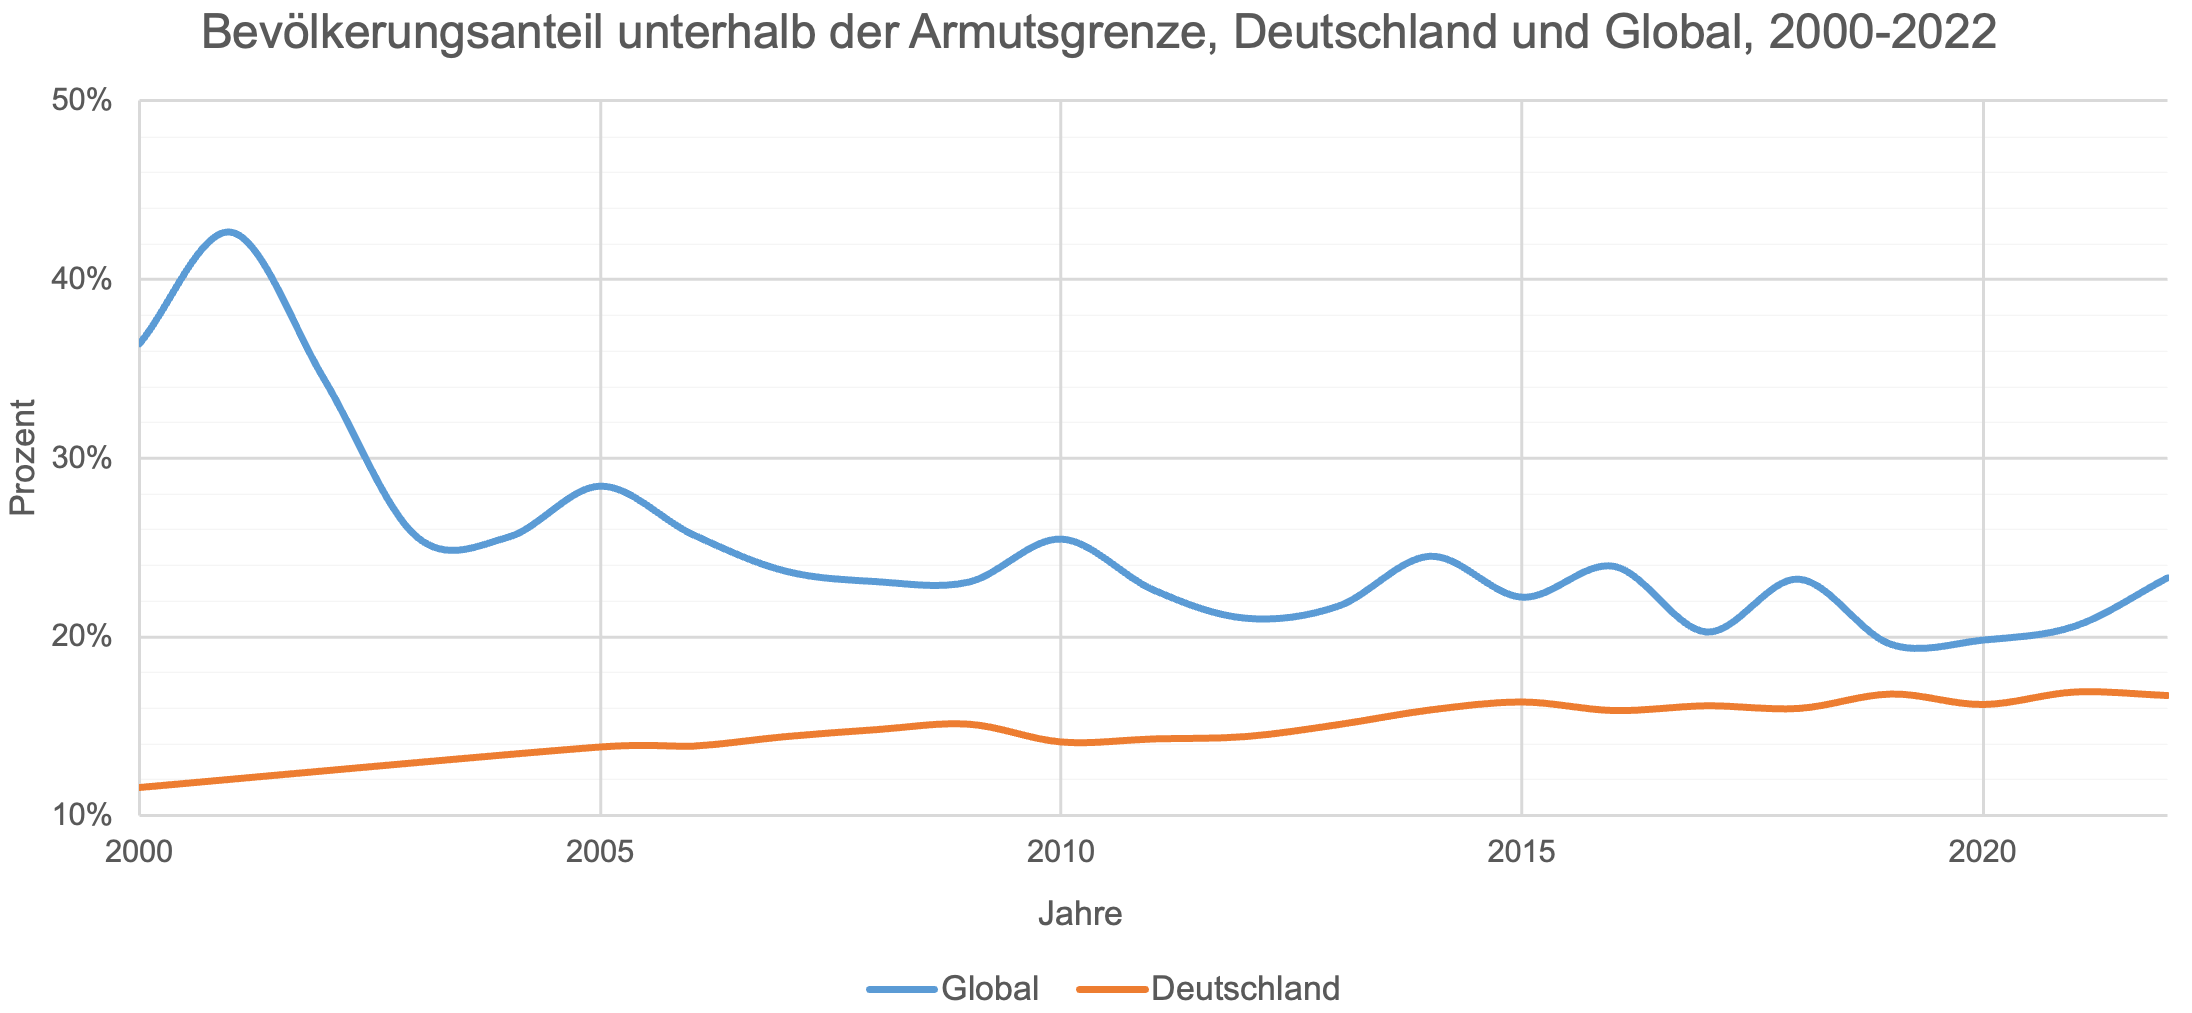
\includegraphics[height=6.9cm]{Bilder/Armutsgrenze2.png}
    \caption[Bevölkerungsanteil unterhalb der Armutsgrenze, Deutschland und global, 2000-2020]{Bevölkerungsanteil mit einem Einkommen unterhalb der Armutsgrenze in Deutschland und auf globaler Ebene von 2000 bis 2020. Eigene Darstellung und Berechnung. Daten abgerufen von \cite[][(global)]{wb_armutsquote_global_2022} und \cite[][(Deutschland)]{bmas_arb_armutsrisikoquote_2023} am 01.03.2024.}
    \label{fig:iso_norm3}
\end{figure}

Das unten aufgeführte Diagramm des Bevölkerungsanteils unterhalb der Armutsgrenze zeigt, dass in Deutschland der Anteil der Bevölkerung der armutsgefährdet ist, von 11\% im Jahr 2000 fast konstant auf ca. 17\% im Jahr 2020 gestiegen ist. Diese Entwicklung kann neben den, bei den anderen Indikatoren bereits genannten Gründen, auch auf die schwache Entwicklung der unteren Einkommen und die gleichzeitige Zunahme der Lebenshaltungskosten zurückgeführt werden. \footcite[Vgl. ][S. 17 (Country-Sheets)]{wir_2022} Ein gro{\ss}er Teil dieser Lebenshaltungskosten sind Mietkosten, welche in gro{\ss}en Städten seit der Jahrtausendwende um teils mehr als 50\% gestiegen sind. \footcite[Vgl. ][S. 494]{kholodilin_mietpreisbremse_2016} Dadurch lässt sich auch erklären, dass die Armutsrisikoquote bei Mietern ca. doppelt so hoch ist, wie beim deutschen Durchschnitt und sechsmal so hoch wie bei Menschen, die in ihrem Wohneigentum leben. \footcite[Vgl. ][S. 458]{grabka_einkommensverteilung_2018}

Auf globaler Ebene lässt sich eine gegensätzliche Entwicklung beobachten: Die Armutsquote ist mit einem Rückgang von ca. 36\% auf 24\% um ein Drittel verringert. Beachtenswert ist hier, dass der Indikator auf globaler Ebene wesentlich stärker als auf deutscher Ebene und als die anderen Indikatoren schwankt bzw. zurückgegangen ist. 

Bei der Gegenüberstellung der beiden Graphen fällt auf, dass der Anteil der Bevölkerung unterhalb der Armutsgrenze in Deutschland im globalen Vergleich zwar etwas geringer ist, die beiden Datenreihen aber wesentlich näher beieinander liegen als es \zB beim Gini-Koeffizient der Fall ist. In Übereinstimmung mit den vorher betrachteten Kennzahlen ist auch hier zu bemerken, dass auf globaler Ebene der Trend in Richtung fallender Armutsquoten geht, während Deutschland  sich eher in die entgegengesetzte Richtung entwickelt. Diese Aussage ist dennoch etwas einzuschränken, da für jedes Land eigene Armutsgrenzen definiert wurden, die auch einen ganz anderen Lebensstandard als in Deutschland abbilden können. Da die Einkommensverteilung mit der Armutsrisikoquote korreliert, lässt sich auch aus diesem Indikator eine steigende Einkommensungleichheit in Deutschland und eine sinkende Einkommensungleichheit auf globaler Ebene ableiten, wenngleich die Einkommensverteilung in Deutschland noch wesentlich ausgeglichener ist, als im globalen Vergleich.

\chapter{Fazit/ Schlussbetrachtung}

Abschlie{\ss}end sollen die in dieser Arbeit gewonnenen Erkenntnisse zusammengefasst werden. Insgesamt haben sich alle betrachteten Kennzahlen auf der Ebene Deutschlands und global über die letzten 25 Jahre hinweg angenähert, was auch auf eine ähnlicher werdende Einkommensverteilung hindeutet. Genauer hei{\ss}t das: Die Einkommen in Deutschland verteilen sich ungleicher, während sich die Verteilung im weltweiten Durchschnitt gleichmä{\ss}iger gestaltet. Als Gründe für diese Entwicklung wurden in Deutschland unter anderem eine gestiegene Arbeitslosigkeit während der 2000er Jahre und der damit einhergehende Ausbau des Niedriglohnsektors, stagnierende Sozialleistungen und wesentlich höhere Zuwanderungsraten identifiziert werden. Die beiden gro{\ss}en Wirtschaftskrisen Anfang der 2000er Jahre und 2008/ 09 haben die Einkommensverteilung in Deutschland und weltweit beeinflusst.

Diese Entwicklungen sollen jedoch nicht über die Tatsache hinwegtäuschen, dass die Einkommensverteilung in Deutschland im internationalen Vergleich immer noch sehr gleichmä{\ss}ig ist, was unter anderem an umfangreichen sozialen Sicherungssystemen und an einer hohen Umverteilung von hohen zu niedrigen Einkommen liegt. Auch wenn sich das deutsche und das internationale Niveau angenähert haben, ist Deutschland hat in absoluten Zahlen eine ausgeglichenere Einkommensverteilung als der internationale Durchschnitt.

Die Betrachtung hat gezeigt, dass die gesellschaftliche Thematisierung wichtig ist, um eine Spaltung der Gesellschaft vorzubeugen. Daher ist es wichtig, dass die Verteilung der Einkommen auf eine Gesellschaft, auch durch politische Ma{\ss}nahmen, in einem gesellschaftsverträglichen Rahmen gehalten wird.